\section{Introduction}

%- cappello introduttivo sulle applicazioni distribuite, e su quali sono i
%rischi correlati (in pratica, i primi due paragrafi in co2-middleware)

Modern distributed applications are often composed 
by loosely-coupled services, 
which can dynamically discover and invoke other services
in order to adapt to changing needs and conditions,
and can appear and disappear from the network. %
These services may be under the governance of mutually distrusting providers 
(possibly competing among each other), 
and interact through open networks, %
where attackers can try to exploit their vulnerabilities. %

In the setting outlined above, % in the previous paragraph, 
developing trustworthy services and applications 
can be a quite challenging task:
the problem fits within the area of computer security,
since we have \emph{adversaries} (in our setting, third-party services),
whose exact number and nature is unknown 
(because of openness and dynamicity). %
%
Further, standard analysis techniques for programming languages
(like \eg, type systems) cannot be applied, 
since they usually need to inspect the code of the whole application,
while under the given assumptions one can only % 
reason about the services under their control. %

\subsection*{Contract-oriented computing}
%Dire che parte dei problemi sopra possono essere affrontati usando i
%contratti. Illustrare concisamente cosa fa un contract-oriented
%middleware. Parlare della reputazione.

A possible countermeasure to these issues is to discipline the interaction
between services through \emph{contracts}.
A contract specifies an abstraction of the intended behaviour of a service,
both from the point of view of what it offers to the other services, 
and of what it requires in exchange.
Services \emph{advertise} contracts when they want to offer 
(or sell) some features to clients over the network, or when 
they want to delegate the implementation of some features to some other services.

The communication is managed by a \emph{contract-oriented middleware}
that plays the role of a trusted party collecting
all the advertised contracts and establishing a \textit{session}
between participants whose contracts are compliant. %
The interaction is \textit{monitored} by the middleware, %
which can blame a participant responsible of
a contract violation, and then suitably punish it. 
% The notion of \emph{reputation} can
% be used to punish a blamed service: whenever a contract is violated,
% the culprit is sanctioned by decreasing its reputation and
% consequently its chances to establish new sessions.

\begin{figure}[t]
  \centering
  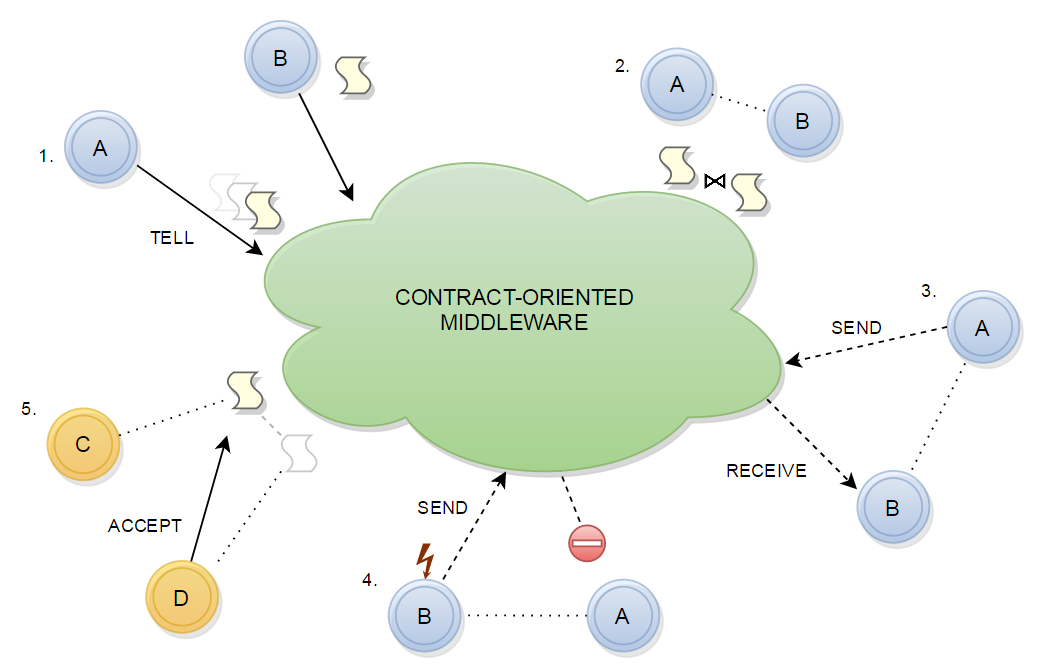
\includegraphics[width=0.8\textwidth]{primitive-schema.png}
  \caption{A schema of the primitive behaviours (from~\cite{CO2}).} 
  \label{fig:primitives}
\end{figure}

\Cref{fig:primitives} illustrates the main features of the middleware
presented in~\cite{CO2middleware}. %
In (1), the participant $\pmv A$ advertises its contract to the middleware, %
making it available to other participants.
%
In (2), the middleware determines that the contracts of 
$\pmv A$ and $\pmv B$ are compliant,
and then it establishes a session through which
the two participants can interact. %
This interaction consists in sending and receiving messages, 
similarly to a standard message-oriented middleware (MOM)~\cite{Banavar99dc}: % 
for instance, in (3) participant $\pmv A$ delivers to the middleware a message for $\pmv B$,
% with the primitive $\send$,
which can then collect it from the middleware.

%The interaction between participants consists in sending and receiving messages, similarly to a standard message-oriented middleware (MOM)\cite{Banavar99dc}: in a established session, a message is delivered to the middleware by a participant and can be collected by the other one. 
Unlike standard MOMs, the interaction happening in each session is monitored by the middleware, 
which checks whether contracts are respected or not. 
In particular, the execution monitor verifies that 
actions can only occur when prescribed by their contracts, %
and it detects when some expected action is missing.

For instance, in (4) the execution monitor has detected  
an attempt of participant $\pmv B$ to do some illegal action. %
Upon detection of a contract violation, the middleware 
punishes the culprit, %
by suitably decreasing its \emph{reputation}. 
This is a measure of the trustworthiness of a participant
in its past interactions: the lower is the reputation,
the lower is the probability of being able to establish new sessions with it.

\subsection*{Analysing contract-oriented services}
%Dire che questo paradigma rende possibile degli attacchi (paragrafi a
%partire da "When the SOC middleware detects contract violations..." in
%50-shades-of-honesty). Concludere dicendo che allo stato attuale manca la
%possibilita' di verificare la honesty dalla specifica all'implementazione.

The sanction mechanism featured by the contract-oriented middleware
allows for a new form of attacks: 
malicious users can try
to make some service sanctioned by exploiting possible discrepancies between
the promised and the actual behaviour of that service. %
A crucial problem is then
how to avoid such attacks \emph{before} deploying a service. %

When services behave in the ``right way'' for all the contracts
they advertise,
they are called \emph{honest}. %
Instead, when services are \emph{not} honest,
they do \emph{not} always respect the contracts they advertise,
at least in some execution context. %
This may happen either unintentionally
(because of errors in the service specification, or in its implementation),
or even because of malicious behaviour.
%However, designing an \emph{honest} service which always respects its contracts requires one to fulfil its obligations also in adversarial contexts which play against.

To study honesty at the specification level we can use \coco, 
a core process calculus for contract-oriented 
computing~\cite{BZ10lics,BTZ12sacs}.

In \coco we formalize services 
as processes that can advertise contracts with the $\tell{}{}$ primitive,
and realize them with the $\fact{}{}$ primitive. %

For example, consider the following \coco process: 
\[
\procP \; = \; (x) \; 
\tell {} {\freeze{x}{\atomIn{a} \sumExt \atomIn{b}}} \cocoSeq \;
\fact x {\atomIn{a}}
\]
The process $\procP$ above advertises the contract 
$\atomIn{a} \sumExt \atomIn{b}$, stating that 
it will receive a message of kind $\atom{a}$ or $\atom{b}$. %
When the contract is stipulated,
the middleware creates a new session $x$, 
and then the service waits to receive through that session 
a message of kind $\atomIn{a}$. %
The process $\procP$ is \emph{dishonest}: 
indeed, if the other participant involved at session $x$ 
sends a message of kind $\atom{b}$,
then $\procP$ is not going to do the corresponding input. %
Note however that $\procP$ is honest in all 
contexts where either the session $x$ is not created,
or the participant at the other endpoint of session $x$ 
never sends messages of kind $\atom{b}$. %

Another (more involved) example is the following:
\[
\procP\; = \; (x, \, y) \;
\tell {} {\freeze{x}{\atomIn{a}}} \cocoSeq \;
\tell {} {\freeze{y}{\atomOut{b}}} \cocoSeq \;
\fact x {\atomIn{a}} \cocoSeq \;
\fact y {\atomOut{b}}
\]

The process $\procP$ advertises two contracts: 
$\atomIn{a}$, which waits for a message of kind $\atom{a}$, 
and $\atomOut{b}$, which  sends a message of kind $\atom{b}$,
respectively on sessions $x$ and $y$. %
When the session $x$ is created, $\procP$ receives a message of kind $\atom{a}$,
and then,  when also $y$ is created, it sends a message of kind $\atom{b}$. %

Surprisingly enough, the process $\procP$ is \emph{dishonest},
for two different reasons.
First, in contexts where session $y$ is created and $x$ is not, 
the $\fact y {\atomOut{b}}$ cannot be reached 
(and so the contract at session $y$ is not fulfilled).
Second, also in those contexts where both sessions are created,
if the other participant at session $x$ never sends the $\atom{a}$ message,
then $\fact y {\atomOut{b}}$ cannot be reached.

The problem of verifying honesty is not trivial, 
also because one must consider \emph{all} possible execution contexts, 
which are infinite. %
Indeed, honesty of \coco processes is \emph{not} decidable, as shown 
in~\cite{Bartoletti15wsfm}. %
Verifying honesty is only possible in non Turing-powerful fragments of \coco,
for instance the one where processes are essentially finite-state,
i.e.\ they have neither delimitation nor parallel under process definitions. %
In this case, it is possible to verify honesty 
by using the model-checking technique of~\cite{verifiable}. %

A further issue is that, 
even if we assume an honest \coco specification, 
it is still possible that honesty no longer holds 
when refining the specification into an actual implementation 
(e.g.\ a Java program using the middleware APIs of~\cite{CO2}). %
% the risk of incurring a sanction at runtime, so preserving the reputation.
% we still need to verify that the corresponding implementation is honest, too. %
% reducing 
%
With the existing techniques developed for \coco, 
one can only check honesty at the level of specification:
this requires a developer to
write a \coco process in the Maude language~\cite{Maude01},
and then by to apply there the model-checking tool of~\cite{verifiable}. %
% However, this is not enough, because errors could be introduced in the implementation, which could break the property.
Analysis techniques for checking honesty at the level of of implementation
are therefore needed in order to develop secure contract-oriented applications.

%He can only check its \coco specification with the model-checker provided in \cite{verifiable}, writing a representation in the Maude language\footnote{Maude is a programming language supporting both equational and rewriting logic specification\cite{Maude01}}.

\subsection*{Contributions}
%Praticamente qui ci va la roba che hai scritto a partire da "This Master’s
%thesis want...". Questa e' la parte piu' importante di tutto il lavoro,
%quindi va fatta con estrema cura. Intanto cerca di omettere le parti piu'
%tecniche (ad es. la roba sul parser non fa parte del contributo
%scientifico del lavoro, quindi andrebbe spostata nei capitoli dove dai i
%dettagli tecnici). Focalizzati invece su quelle metodologiche: 

%Cosa ci guadagna lo sviluppatore nell'usare i tuoi tool? Come li hai validati? 
%Il paradigma e' abbastanza generale da essere utile in scenari concreti? 
%Gli strumenti di analisi sono sufficientemente precisi? (qui devi rimarcare che li hai testati on successo su una suite di casi di studio).
%Sono sufficientemente efficienti? 
%Insomma, tutto quello che si puo' dire di positivo su quello che hai fatto, va scritto qui.

We provide a support to programmers on the development of contract-oriented 
applications. 
In order to do so, we develop an Eclipse plugin that allow to write \coco processes, verify their honesty, and automatically generate skeletons of Java programs that interact using the above mentioned contract-oriented middleware.

The possibility of auto-generating Java code from a \coco process simplifies and speeds up the development of a distributed application.
Without using our tools, a possible approach can be:
\begin{enumerate}[(i),topsep=5pt,itemsep=1pt,parsep=0pt]
	\item\label{step:1} write the \coco process that models the application;
	\item\label{step:2} write the Maude program to model-check the specification;
	\item\label{step:3} repeat steps \textit{\ref{step:1}} and \textit{\ref{step:2}} until the process becomes honest;
	\item\label{step:4} implement the process using an high-level language (\eg Java).
\end{enumerate}
Considering that there is not any tool to support steps \textit{\ref{step:1}} and \textit{\ref{step:2}}, this methodology is tedious and wasteful. For example, consider the case in which a specification changes: the first three steps must be repeated and the implementation modified accordingly. 
Since software specifications change quite often, 
this leads to poor maintainability of any non trivial application. %
Furthermore, there is no check that validates the implementation 
resulting from step \textit{\ref{step:4}}.

We simplify the overall process. %
Our plugin speeds up the writing of \coco processes, 
reducing the time spent on step \textit{\ref{step:1}}. 
Step \textit{\ref{step:2}} is completely removed (the Maude program is auto-generated, so the knowledge of another language is not needed), 
and step \textit{\ref{step:3}} changes accordingly. %

The main contribution is made on step \textit{\ref{step:4}}: the Java application is automatically generated, 
and it can be modified by the programmer to add any further logic to it, 
maybe making it dishonest. 
We provide a verification technique that allows to skip steps \textit{\ref{step:1}}\textit{\ref{step:2}}\textit{\ref{step:3}} and to directly write distributed contract-oriented application whose
honesty can be checked from the implementation.

Our methodology is validated against three use cases:
\begin{description}

\item[Online store:] 
  a store advertise a contract to interact with buyers. 
  This example, deliberately simple to explain in detail 
  all the verification phases, 
  shows how a \coco specification is translated to Maude and in Java, 
  and how honesty of the Java application is checked.
  
\item[Voucher distribution system:] this example involves multiple sessions 
  and demonstrate the benefit of our work. 
  First, we provide an honest specification of the process, 
  showing that both Maude and Java programs respond in the same way. 
  Then, we change our specification into a dishonest one:
  our verification technique correctly detects that 
  the corresponding Java program is dishonest as well.
	
\item[Blackjack:] the last example shows how a specification can be difficult to write and maintain. The advertised contracts are both recursive and the specification is split into different parts due to its complexity. There are also multiple sessions, parallel processes, if-then-else selection and recursive behaviour.
\end{description}

Our tool allows to change the specifications \emph{on-the-fly} and immediately verify if the changes are good or not. 
Also, considering the total time spent to check the honesty is in the order of few hundred of milliseconds, there is no additional overhead on development.

\subsection*{Structure of the paper}

The paper is organised as follows: \Cref{sec:back} presents a brief overview of the background theory and tools already presents;
%  describe the Eclipse plugin and the verification strategy adopted for Java programs.
\Cref{sec:co2-to-java} shows the transformation from \coco processes
to Java programs and it presents the \coco Eclipse plugin;
\Cref{sec:java-honesty} explains how we verify honesty of Java
programs;  \Cref{sec:validation} validates the effectiveness of out
tools, by applying them to some use cases; finally,
\Cref{sec:conclusions} summarizes the reached goals and proposes
possible evolutions of our work.


\subsection{Objectives}
 Di fatto i tool sono 3:
 
 1. model-checker maude
 
 2. model-checker java
 
 3. eclipse plugin

 la cui dipendenza è 1 $\longleftarrow$ 2 $\longleftarrow$ 3
 
 Gli obbiettivi che vogliamo raggiungere sono
 
 - semplificare la scrittura di processi co2 (plugin eclipse)
 
 - automatizzare la scrittura di codice maude per la verifica di onestà della specifica co2 (plugin eclipse)
 
 - automatizzare la scrittura di codice java che rispetti la specifica co2 (plugin eclipse)
 
 - verificare l'onestà di programmi java (tool java)

 Descrivere a chi sono rivolti i tool.


I tool sono rivolti a due tipi di utenti:
- utenti esperti: hanno conoscenza di \coco e hanno familiarità nella scrittura
di processi utilizzando le specifica, conoscono nel dettaglio la semantica e le
proprietà di onestà e colpevolezza;
- utenti base: conoscono il paradigma contract-oriented ad un livello astratto 
ignorando il modello formale; hanno un'idea generica di cosa sià l'onestà 
e la colpevolezza
